\documentclass[11pt,a4paper]{article}
\usepackage[ngerman]{babel}
\usepackage[utf8]{inputenc}
\usepackage{geometry}
\usepackage{subfig}
\usepackage{nicefrac} 
\usepackage{amssymb}
\usepackage{mathrsfs} 
\usepackage{graphicx}
\usepackage{paralist}
\addto\captionsngerman{\renewcommand\figurename{Abb.}}
\usepackage{amsmath}
\usepackage[headsepline,nouppercase]{scrpage2}
%%\usepackage[headsepline,plainheadsepline]{scrpage2}
\usepackage{setspace}
\author{Philipp Wilhelm Klein}
\date{}
\title{Chaos in klassischer (Hamilton'scher) Dynamik\bigskip\\ \large Arbeitsgruppe III: \hspace{0.3cm}Zufall und Komplexität in der Physik}
\geometry{a4paper,left=3cm, right=3cm, includeheadfoot, top=2cm,bottom=2cm}



\pagestyle{scrheadings}
\ihead[\rightmark]{\rightmark} \chead[]{}
%\ohead[\pagemark]{\pagemark} \cfoot[]{}
\automark{section}


\begin{document}

\maketitle 
\renewcommand{\contentsname}{Inhalt}
\tableofcontents
\thispagestyle{empty}



\section{Die Poincar\'{e} Abbildung}
\subsection{Die \grqq Surface of Section\grqq}


\textbf{Vorbemerkung.} Im folgenden werden wir der Einfachheit bzw. Anschaulichkeit halber integrable, Hamilton`sche Systeme mit 2 Freiheitsgraden betrachten.
\\
\\
Grundsätzlich ist die Veranschaulichung dynamischer (Hamiltion'scher) Systeme aufgrund der Dimension des Phasenraums (dieser ist für ein System mit $ n $ Freiheitsgraden $ 2n $-dimensional) nicht möglich. Für ein konservatives, dynamisches System mit 2 Freiheitsgraden \grqq lebt\grqq die Hamilton-Funktion auf einer 3-dimensionalen Hyperebene im 4-dimenionalen Phasenraum (siehe Abb.~\ref{3dim-Hyperebene}).
\begin{figure}[h]
\centering
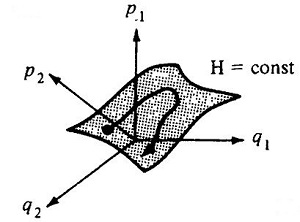
\includegraphics[width=5cm]{3dim-Hyperebene-4dim-PR}
\caption{3-dim Hyperebene im 4-dim Phasenraum, Quelle: \cite{LL}}
\label{3dim-Hyperebene}
\end{figure}
Anstatt eine Trajektorie (die in der Hyperebene liegt) als Ganzes zu studieren, fixiert man einen Parameter ($ q_2=0 $) und betrachtet Transversalschnitte der Trajektorie mit einer 2-dim. Ebene im Phasenraum (siehe Abb.~\ref{SOS})
\begin{figure}[h]
\centering
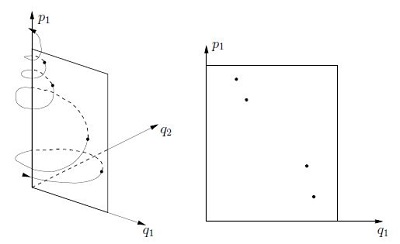
\includegraphics[width=8cm]{SOS}
\caption{Surface of Section (SOS), Quelle: \cite{Wim}}
\label{SOS}
\end{figure}
\newline Dies motiviert folgenden Defintion.
\newline
\newline
\textbf{Defintion.} Die \textit{Surface of Section (SOS)} ist unter den obigen Voraussetzungen die Menge
\begin{equation*}
SOS = \lbrace \left( q,p\right)\in\mathbb{R}^4\hspace{0,1cm}\vert \hspace{0,1cm} q_2=0, H(q,p)=E\rbrace
\end{equation*}

\subsection{Die Poincar\'{e} Abbildung}
\textbf{Definition.} Sei $ \varphi $ eine Trajektorie mit den Anfangsbedingung $ (q_0,p_0)\in SOS $, die nach der Reihe die Punkte $ (q_1,p_1),(q_2,p_2),\ldots \in SOS $ durchläuft. Dann ist die \textit{Poincar\'{e} Abbildung} $ \mathcal{P} $ definiert durch \[ \mathcal{P}: (q_i,p_i)\longmapsto \mathcal{P}_i(q_0,p_0) = (q_{i+1},p_{i+1})\]
\begin{figure}[h]
\centering
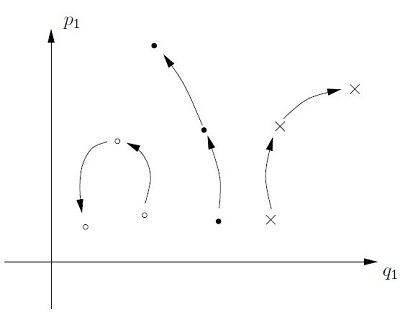
\includegraphics[width=8cm]{PoinMap}
\caption{Die Poincar\'{e} Abbildung für drei verschiedene Startpunkte einer Trajektorie auf der SOS, Quelle: \cite{Wim}}
\label{PoinMap}
\end{figure}
\newline
Eine wichtige Aussage über die Entwicklung von Transversalschnitten von Flußbildern in Hamilton'schen Systemen macht der folgende Satz.
\newline
\newline 
\textbf{Satz.} (Poincar\'{e}-Cartan) Die Poincar\'{e} Abbildung ist Flächenerhaltend. Genauer: Sei $ \sigma_0\subset SOS $ in der $ \left q_1p_1$-Ebene. Sei $ \sigma_i=\mathcal{P}_i(\sigma_0) $ die Menge, die nach $ i $-facher Anwendung der Poincar\'{e} Abbildung $ \mathcal{P} $ auf $ \sigma_0 $ entsteht. Dann gilt:  \[\vert \sigma_i \vert = \vert \sigma_0 \vert\] 
\begin{figure}[h]
\centering
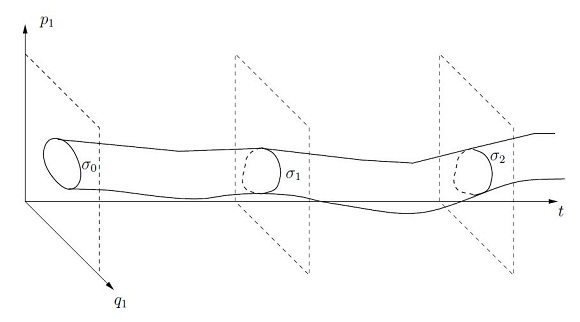
\includegraphics[width=9cm]{PoinCart}
\caption{Veranschaulichung des Satzes von Poincar\'{e}-Cartan: Es gilt $ \vert \sigma_0 \vert = \vert \sigma_1 \vert = \vert \sigma_2 \vert = \ldots $, Quelle: \cite{Wim}}
\label{PoinMap}
\end{figure}


\section{Fixpunkte}
\textbf{Definition.} Ein Fixpunkt der Poincar\'{e} Abbildung $ \mathcal{P} $ ist definiert durch \[\mathcal{P}(z^*)=z^*\] mit $ z^*=(q^*,p^*) \in SOS $.
\newline
\newline
\textbf{Linearisierung in einer Fixpunktumgebung.} Sei $ z^* \in SOS $ Fixpunkt der Poincar\'{e} Abbildung $ \mathcal{P} $. Dann lässt sich $ \mathcal{P}(z^*) $ in einer Umgebung von $ z^* $ approximieren durch \[ \mathcal{P}(z^* + \delta z) = z^* + d\mathcal{P}(z^*)\cdot \delta z\ + \mathcal{O}(\delta z^2),\] wobei $ \mathcal{M} \equiv \mathcal{M}(z^*) = d\mathcal{P}(z^*) $ die Jakobimatrix der Abbildung $ \mathcal{P} $ ist.
\\
\\
\textbf{Klassifikation von Fixpunkten.} Die Eigenschaften des Fixpunktes werden bestimmt durch die Eigenwerte der Matrix $ \mathcal{M} $. Also führt $ det( \mathcal{M} - \lambda) = 0 $ zu\[ \lambda^2 - \lambda tr( \mathcal{M}) + det( \mathcal{M}) = 0, \] wobei $ det( \mathcal{M}) = 1$ sein muss, da $ \mathcal{P} $ flächenerhaltend ist. Die Eigenwerte lauten also \[ \lambda_{1,2} = \frac{1}{2}tr( \mathcal{M}) \pm \frac{1}{2}\sqrt{tr( \mathcal{M})^2 -4 }, \] und können in Abhängigkeit von $ tr( \mathcal{M}) $ klassifiziert werden. Es ergeben sich folgende Fälle:
\begin{compactenum}[(i)]
\item $ \vert tr( \mathcal{M})\vert < 2  $: Die Eigenwerte sind komplexe Zahlen und lassen sich mithilfe der Exponentialfunktion ausdrücken, d.h. $ \lambda_{1,2} = \exp(\pm i \beta) $ mit $ \beta \in (0,\pi) $.
In diesem Fall ist $ \mathcal{M} $ eine Rotationsmatrix, d.h. in der direkten Umgebung des Fixpunktes $ z^* $ verhält sich $ \mathcal{P} $ wie eine Rotationsabbildung. Damit ist das dynamische System in der Umgebung von  $ z^* $ stabil, siehe Abb.~\ref{klassfixp}(a). Man spricht von einem \textit{elliptischen Fixpunkt}.
\item $ \vert tr( \mathcal{M}) \vert > 2 $: Die Eigenwerte sind reel und haben die Form $ \lambda_1 = \lambda $ bzw. $ \lambda_2 = \frac{1}{\lambda} $. In diesem Fall ergibt sich ein \textit{hyperbolischer Fixpunkt}, siehe Abb.~\ref{klassfixp}(b). Dieser Fixpunkt ist damit instabil.
\item $ \vert tr( \mathcal{M}) \vert = 2 $: Dieser Fall kennzeichnet den Grenzfall zwischen Stabilität bzw. Instabilität.
\end{compactenum}
\begin{figure}[h]
\centering
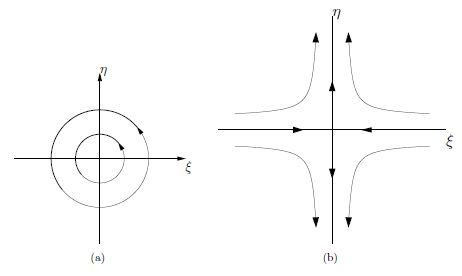
\includegraphics[width=10cm]{klassfixp}
\caption{Verhalten dynamischen Systems in der Nähe eines elliptischen (a) bzw. hyperbolischen (b) Fixpunktes, Quelle: \cite{Wim}}
\label{klassfixp}
\end{figure}
\textbf{Beispiel.} Wir betrachten ein System mit folgender Hamiltonfunktion:
\[ H = \frac{p^2}{2} + (q^2 - 1)^2. \]
Das Potential $ V(q) $ veranschaulicht Abb.~\ref{bspfixp}a. Das System hat drei Fixpunkte: zwei stabile Minima $ (s) $ (elliptisch) und ein instabiles Maximum $ (i) $ (hyperbolisch). Dies ist zunächst anhand der Form des Potentials anschaulich klar und wird durch das Phasenraumbild belegt, siehe Abb.~\ref{bspfixp}b.
\begin{figure}[h]
\centering
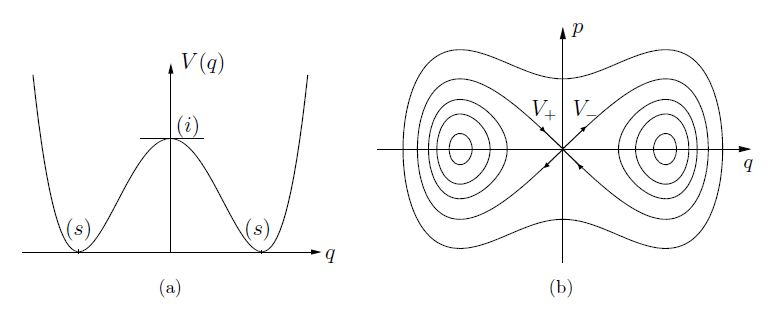
\includegraphics[width=10cm]{bspfixp}
\caption{(a) stellt qualitativ das Potential dar, (b) zeigt das zugehöre Phasenraumbild, Quelle: \cite{Wim}}
\label{bspfixp}
\end{figure}


\section{Der Satz von Poincar\'{e}-Birkhoff }

\textbf{Erinnerung.} (KAM-Theorem) Phasenraumkurven mit irrationaler Rotationszahl (d.h. $ \frac{\omega_1}{\omega_2} \equiv \alpha \in \mathbb{R}\backslash\mathbb{Q}) $ weichen für hinreichend kleine Störungen nur leicht von ihrer ungestörten Bahn ab (solange die Bedingung $ \mathrm{det}\left( \frac{\partial \omega(J)}{\partial J}\right) \right\vert_{J\approx I} \neq 0 $ erfüllt ist). Was irrationale Rotationszahl bedeutet, veranschaulicht Abb.~\ref{torusirra}.
Eine Aussage über Trajektorien mit rationaler Rotationszahl ($ \alpha \in \mathbb{Q} $), siehe Abb.~\ref{torusra}, liefert im Folgenden der Satz von Poincar\'{e}-Birkhoff. 
\begin{figure}[h]
\centering
\hfill %
\subfloat[ \label{torusirra}]{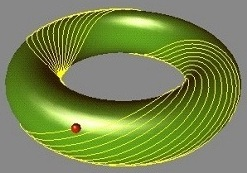
\includegraphics[width=6cm]{torusirra}}
\hfill %\hspace{1cm} 
\subfloat[ \label{torusra}]{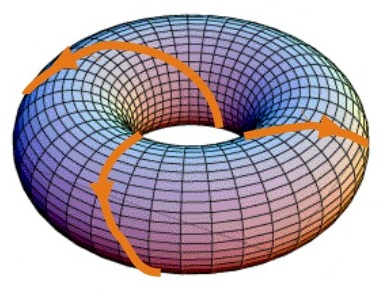
\includegraphics[width=5cm]{torusra}}
\hfill %
\caption{Trajektorie auf Torus: mit irrationaler (a) bzw. rationaler (b) Rotationszahl}
\label{Gesamtbild}
\end{figure}
\newline
\newline
\textbf{Beobachtung.} Sei $ H(I_1, I_2,\Theta_1, \Theta_2 )= H_0(I_1,I_2) + \epsilon H_1(I_1,I_2,\Theta_1,\Theta_2)  $ die Hamiltonfunktion, bestehend aus einem integrablen Teil $ H_0 $, der mit Wirkungs-Winkel-Variablen beschreibbar ist und einem (kleinen) Störtherm $ \epsilon H_1 $. Eine ungestörte Trajektorie verläuft auf einem Torus im 4-dimensionalen Phasenraum. Ihre Poincar\'{e}-Abbildung hat die Form $ \Theta_1^{'} = \Theta_1 + 2\pi\cdot \alpha(I_1) $ und $ I_1  $ bleibt unverändert, d.h. $ I_1^{'} = I_1 $. Dabei soll $ \alpha $ gleichmäßig von $ I_1 $ abhängen und es gelte $ \alpha = \frac{m}{n} $, wobei $ m $ und $ n $ teilerfremde ganze Zahlen sind.

Sei nun $ \mathcal{C} \subset SOS $ ein $ \mathcal{P} $-invarianter Kreis in der SOS, d.h. es gilt $ \mathcal{P}(\mathcal{C})=\mathcal{C} $, wobei das dynamische Verhalten der Punkte in $ \mathcal{C} $ durch $ \alpha(I_1) $ beschrieben wird. Wenn wir nun $ I_1 $ größer oder kleiner wählen, finden wir Kreise $ \mathcal{C^+} $, bzw. $ \mathcal{C^-} $, die außerhalb bzw. innerhalb von $ \mathcal{C} $ liegen und irrationale Rotationszahlen haben.  Da $ \alpha $ gleichmäßig von $ I_1 $ abhängt, rotiert, in Bezug auf $ \mathcal{C} $, $ \mathcal{C^+} $ im Uhrzeigersinn und $ \mathcal{C^-} $ gegen den Uhrzeigersinn wenn man ihre Punkt $ n $-fach unter $ \mathcal{P} $ iteriert, siehe Abb.~\ref{poinbi1}a.
\begin{figure}[h]
\centering
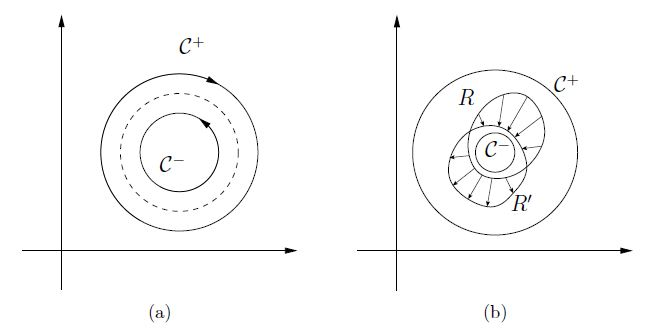
\includegraphics[width=10cm]{poinbi1}
\caption{(a) zeigt die Kreise $ \mathcal{C} $ (gestrichelt), sowie außer- bzw. innerhalb $ \mathcal{C^+} $ und $ \mathcal{C^-} $ auf der SOS, Quelle: \cite{Wim}}
\label{poinbi1}
\end{figure}

Nun betrachten wir die Veränderungen unter Einfluss des Störtherms $ \epsilon H_1 $. Die zum gestörten System gehörige Poincar\'{e} Abbildung bezeichnen wir mit $ \mathcal{P^\epsilon} $. Nach dem KAM-Theorem wirkt sich der Störtherm auf $ \mathcal{C^+} $ und $ \mathcal{C^-} $ kaum aus, d.h. sie sind invariant unter $ \mathcal{P^\epsilon} $. Wir nehmen außerdem an, dass $ \epsilon $ so klein gewählt ist, dass sich der relative Drehgeschwindigkeit unter $ \mathcal{P}^\epsilon_n $ nicht (bzw. kaum) ändert. Daraus folgt aber direkt schon, dass für jeden Radius zwischen den Radien von $ \mathcal{C^+} $ und $ \mathcal{C^-} $ ein Punkt existiert, dessen Winkelkorrdinate $ \Theta_1 $ unter $ \mathcal{P}^\epsilon_n $ erhalten bleibt. Für jeden Radius aufgetragen formen diese Punkte eine Kurve $ \mathcal{R} $, siehe Abb.~\ref{poinbi1}b. In Abb.~\ref{poinbi1}b ist außerdem die Kurve $ \mathcal{R}^{'} = \mathcal{P}^\epsilon_n ( \mathcal{R} )  $ eingezeichnet. D.h. nach $ n $-facher Anwendung von $ \mathcal{P}^\epsilon $ sind genau die Punkte Fixpunkte von $ \mathcal{P}^\epsilon $, die sich in der Menge $ \mathcal{R} \cap \mathcal{R}^' $ befinden. Diese Fixpunkte treten immer in Paaren auf.

Dies führt schlussendlich auf folgenden Satz.
\newline
\newline
\textbf{Satz.} (Poincar\'{e}-Birkhoff) Sei $ \mathcal{C} \subset SOS $ Kurve eines ungestörten Hamilton`schen Systems mit Rotationszahl $ \alpha = \frac{m}{n} $, die Fixpunkte von $ \mathcal{P}_n $ sind, d.h.:\[ \forall c \in \mathcal{C}: \mathcal{P}_n(c) = c.\] Unter Einfluss eines Störtherms bleiben dann \[ 2kn, \hspace{0.4cm} k \in \mathbb{N}, \] Fixpunkte von $ \mathcal{P} $ erhalten.



\section{Lyapunov-Exponenten, Stabilitätskriterien}

\subsection{Der maximale Lyapunov-Exponent}

\textbf{Beispiel.} Wir betrachten wiederrum ein Hamilton'sches System mithilfe einer Poincar\'{e} Abbildung $ \mathcal{P} $ auf einer SOS. Sei $ z^* \in SOS $ einer hyperbolischer Fixpunkt. Wir möchten die Matrix $ \mathcal{M}_{n}(z^*) $ der Abbildung $ \mathcal{P}_n $ bestimmen. Diese ergibt sich zu $ \mathcal{M}_n(z^*) = \mathcal{M}^n (z^*) $. Seien nun $ \lambda > 1 $ und $ \frac{1}{\lambda} < 1  $ Eigenwerte von $ \mathcal{M} $, dann sind $ \lambda^n $ und $ \frac{1}{\lambda^n} $ Eigenwerte von $ \mathcal{M}_n $. Sei weiterhin $ \mathcal{B}^{'} = \left\lbrace v_1,v_2 \right\rbrace  $ eine Basis aus Eigenvektoren (jeweils zu den Eigenwerten $ \lambda_1 $ bzw. $ \lambda_2 $).

Wir betrachten nun das Verhalten von $ \xi = z^* + \delta z $, d.h. eines Punktes in der Fixpunktumgebung, unter der Abbildung $ \mathcal{P}_n $. Wenn wir noch $ \delta z $ bezüglich der Basis  $ \mathcal{B}^' $ durch $ \delta z = \mu_1 v_1 + \mu_2 v_2 \equiv \delta z_1 + \delta z_2 $ ausdrücken, ergibt sich in linearer Näherung
\begin{eqnarray}
\mathcal{P}_n ( \xi ) & = & z^* + \mathcal{M}_n \cdot \delta z + \mathcal{O}(\delta z^2 ) \nonumber \\
 & = & z^* + \lambda^n \cdot \delta z_1 + \frac{1}{\lambda^n} \cdot \delta z_2 + \mathcal{O}(\delta z^2) \nonumber \\
 & = & z^* + e^{n \ln(\lambda)} \cdot \delta z_1 + e^{-n \ln(\lambda)} \cdot \delta z_2 + \mathcal{O}(\delta z^2). \nonumber 
\end{eqnarray} 
Für hinreichend großes $ n $ ist $ e^{-n \ln(\lambda)} $ entsprechend klein und kann vernachlässigt werden. Damit wird der Abstand eines Punktes $ \xi $ zum Fixpunkt $ z^* $ nach $ n $-facher Anwendung von $ \mathcal{P} $ durch $ \Vert e^{n \ln(\lambda)} \cdot \delta z_1 \Vert $ bestimmt. \\
Man nennt $ \pm \ln(\lambda) $ die \textit{Lyapunov-Exponenten} der Abbildung $ \mathcal{P} $ im Punkt $ z^* $. 
\\
\\
\textbf{Bemerkung.} Das obige Beispiel zeigt, dass zur Überprüfung der Stabilität von Trajketorien der größte Lyapunov-Exponent maßgebend ist. Man nennt diesen auch \textit{maximalen Lyapunov-Exponenten}. Er gibt die Rate an mit der sich zwei Trajektorien voneinander entfernen (bzw. aneinander annähern). Das motivert folgende Defintion:
\\
\\
\textbf{Defintion.} (maximaler Lyapunov-Exponent) Der maximale Lyapunov-Exponent $ \sigma(z) $ der Poincar\'{e} Abbildung $ \mathcal{P} $ (für eine Anfangsbedingung $ z $) ist definiert durch 
\[\sigma(z) \equiv \lim_{n \to \infty} \lim_{\delta z \to 0} \frac{1}{n} \ln \left(  \dfrac{\Vert \mathcal{P}_n ( z + \delta z ) - \mathcal{P}_n (z) \Vert}{\Vert \delta z \Vert } \right).  \]


\subsection{Das Lyapunov-Spektrum}

\textbf{Bemerkung.} Möchte man Wachstumsraten für die Abstände von Trajektorien in allen Phasenraumrichtungen betrachten, so ist es sinnvoll, nicht nur einen, d.h. den maximalen, Lyapunov-Exponenten zu berechnen, sondern jeweils einen für jede Raumrichtung.
\\
\\
\textbf{Definition.} (Lyapunov-Spektrum für $ 2 $-dim. Poincar\'{e} Abbildung $ \mathcal{P} $) An das Beispiel zu Anfang von Kapitel 4.1 anknüpfend, ist das Lyapunov Spektrum gegeben durch
\begin{eqnarray}
\sigma_{1,2}(z) & \equiv & \lim_{n \to \infty} \lim_{h \to 0} \frac{1}{n} \ln \left(  \dfrac{\Vert \mathcal{P}_n ( z + h v_{1,2} ) - \mathcal{P}_n (z) \Vert}{\vert h \vert } \right)   \hspace{0,6cm} (\ast) \nonumber  \\
& = & \ln (  \lambda_{1,2} ). \nonumber
\end{eqnarray}
\\
\\
\textbf{Bemerkung.}Das Beispiel aus Kapitel 4.1 bezog sich auf einen hyperbolischen Fixpunkt. In dessen Nähe stimmt das Lyapunov-Spektrum mit den Eigenwerten der Matrix $ \mathcal{M} $ überein. Das Lyapunov-Spektrum bezogen auf die Zeitentwicklunsfunktion $ \mathscr{H}_t $ des gesamten dynamischen Systems ist analog definiert.



\begin{thebibliography}{xxxxxxxxxxxxxxxxxxx}
   \bibitem[1]{Wim} S. Wimberger, \textit{Nonlinear Dynamics and Quantum Chaos} (2012)
   \bibitem[2]{Tab} M. Tabor, \textit{Chaos and Integrability in Nonlinear Dynamics} (John Wiley & Sons, 1989)
   \bibitem[3]{LL} A.J. Lichtenberg, M.A. Lieberman, \textit{Regular and Chaotic Dynamics} (Springer Verlag, Berlin, 1992)
   \bibitem[4]{Blog} Science-Blogs: http://www.scienceblogs.de/astrodic-ticum-simplex/2009/05/chaotische-systeme-teil-2-der-raum-als-donut.php
\end{thebibliography}



\end{document}